\documentclass{article}
\usepackage{amsrefs}
\usepackage{amssymb}
\usepackage{amsmath}
\usepackage{amsthm}
\usepackage{graphicx}

\DeclareMathOperator{\dom}{dom}
\newtheorem*{definitie}{Definitie} \newtheorem*{notatie}{Notatie} \newtheorem*{voorbeeld}{Voorbeeld} \newtheorem*{eigenschap}{Eigenschap}

\title{Afgeleide en verloop van een functie}
\date { }

\begin{document}

\maketitle \noindent

\noindent Je weet dat $Df(a)$ aangeeft met welke snelheid functiewaarden veranderen als $x$ vanuit $x=a$ verandert.
Als $Df(a)<0$ dan is dat met een negatieve snelheid. Wat betekent dat?\vspace{5mm}

\noindent Dit betekent dat de functiewaarde $f(x)$ afneemt als je start met $x=a$ en dan $x$ laat toenemen.
Dit komt overeen met de volgende figuur.
\begin{figure}[h]
\begin{center}
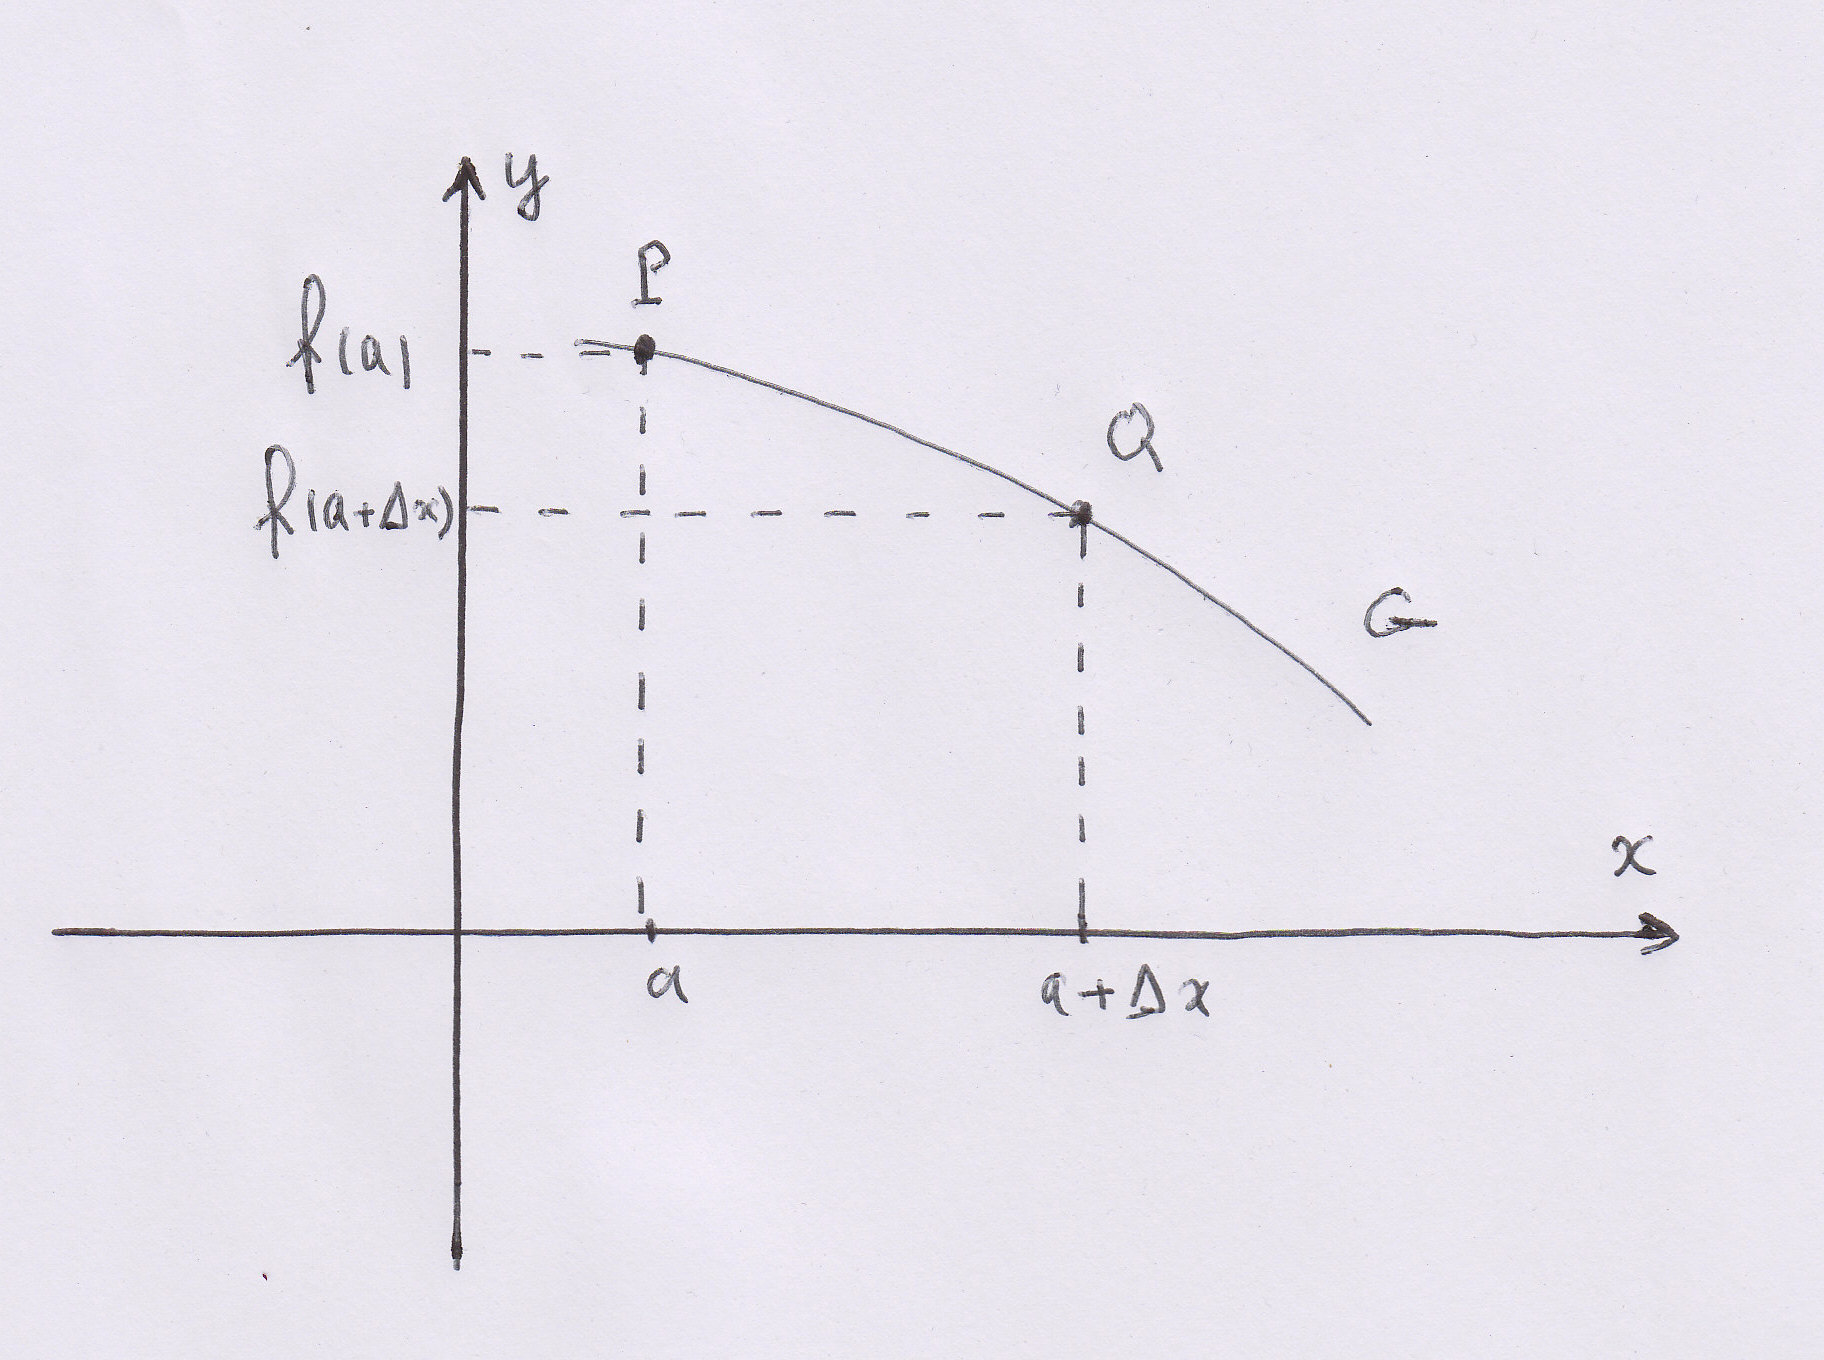
\includegraphics[height=5 cm]{dalend.JPG}
\end{center}
\end{figure}

\noindent In zulk geval heet de functie $f$ dalend in $a$.\vspace{5mm}

\noindent Op dezelfde manier bekom je dat als $Df(a)>0$ dan is de functie stijgend in $a$.
Je bekomt de volgende verbanden tussen $Df$ en het verloop van $f$.

\begin{eigenschap}
Hier komen de eigenschappen uit de kader blz. 15 van de Actimath cursus deel 6.2; het deel op bladzijde 16 hoeft er niet bij.
\end{eigenschap}

\begin{voorbeeld}
het voorbeeld $f(x)=x^3-3x^2$ dat uitgewerkt is in de actimath cursus.
\end{voorbeeld}


\end{document}